% GRtoolbox chapter for GRASP manual
% $Id: man_GRtoolbox.tex,v 1.3 1999/09/06 17:37:17 ballen Exp $
%
% Steve Drasco
% Summer 1998

\section{Matlab Interface: Gravitational Radiation Toolbox}
\label{s:GRtoolbox}
\setcounter{equation}0

The Gravitational Radiation Toolbox provides a
Matlab interface to both GRASP and the Frame Library. 
The toolbox consists of Matlab m-files and mex-files. The m-files are written
in Matlab's native language and are interpreted. The mex-files are written in
C and are compiled. The mex-files take input from the user via Matlab and
then format it and pass it to the corresponding GRASP routine. The GRASP
output is then formatted and passed back into Matlab. The function names and
calling methods have been made to resemble those of their corresponding GRASP
functions with the main difference being that the Matlab user need not be
concerned with memory management and pointers. These functions can be used
from the command line, within other m-files, or via a GUI front end called
\texttt{GRtool}. Currently the toolbox addresses only the detection and simulation
of gravitational radiation from binary inspirals.

When installing GRASP you have the option of installing the Gravitational 
Radiation Toolbox as well. If you have not done this see sections 
\ref{sss:GRtoolboxInstall} and \ref{ss:buildit}
for installation instructions.
\clearpage

\subsection{Using {\tt GRtool}}
\label{ss:GRtool}

The easiest way to test out the toolbox is by using the GUI \texttt{GRtool}.
Once you have successfully installed the toolbox, typing \texttt{GRtool} at
the Matlab prompt should produce the window shown in figure \ref{f:startup}. At
the left of the figure are axes upon which time and frequency domain data can
be displayed. At start-up the only options are to \texttt{Read} or
\texttt{Simulate} data.

%%%%%%%%%%%%%%%%%%%%%%%%%%%%%%%%%%%%%%%%%%%%%%%%%%%%%%%%%%%%%%%%%%%%%%%%%%%%%
%startup.gif
\begin{figure}[h]
\index{colorpage}
\begin{center}
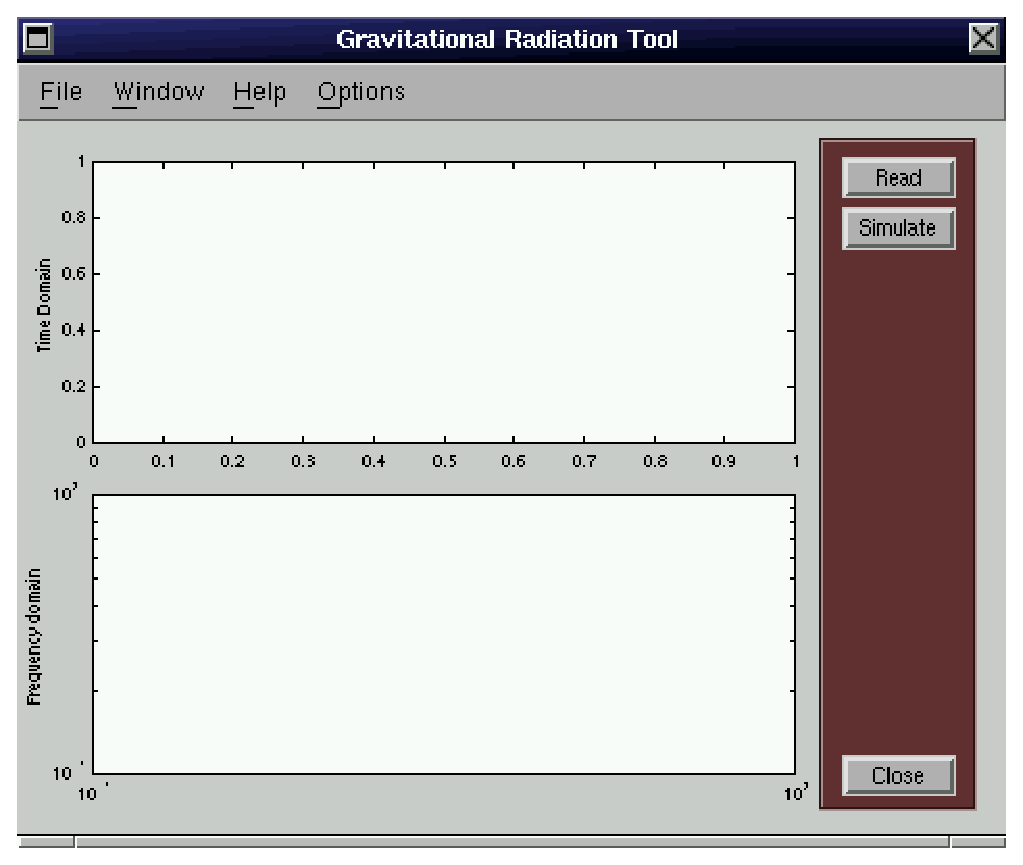
\epsfig{file=Figures/fig_startup.eps,width=6in}
\caption{ \label{f:startup}
The \texttt{GRtool} start-up window}
\end{center}
\end{figure}
%%%%%%%%%%%%%%%%%%%%%%%%%%%%%%%%%%%%%%%%%%%%%%%%%%%%%%%%%%%%%%%%%%%%%%%%%%%%%

If you press \texttt{Simulate} you will enter the simulation GUI from
which you can simulate inspirals up to second post-Newtonian order
approximations as described in \cite{biww} and \cite{willwiseman}.
(Note: You
can always run the simulation GUI alone by entering
\texttt{GRtool('simulate\_build')} at the Matlab prompt.)
 All simulations
are done via a function \texttt{mxMake\_filters} which is a Matlab version of the
function \texttt{make\_filters}. The operation of the simulation GUI is
straightforward. You can plot the time and frequency domain simulations, play
them as sound, or export them to either the Matlab workspace or 
\texttt{*.au} sound files.

If you press \texttt{Read} you will be asked a series of questions. At first
you will be asked if you would like to read from local disks or from a URL. If
you choose local disk, you will then be asked what file you want to open. Only
frame formatted data files with the LIGO\ gravity wave channel
(\texttt{IFO\_DMRO}) can be read---this goes for data read from a local disk
or a URL. If you choose URL you will be prompted for a URL address. After
providing the URL you will be asked where you would like to write the contents
of the URL. When the program has read the data you will be presented with more
buttons on the panel to the right.

Figure \ref{f:tfspace} shows the results of a successful read of a frame file.
%%%%%%%%%%%%%%%%%%%%%%%%%%%%%%%%%%%%%%%%%%%%%%%%%%%%%%%%%%%%%%%%%%%%%%%%%%%%%%%%
%tfspace.gif 
\begin{figure}[h]
\index{colorpage}
\begin{center}
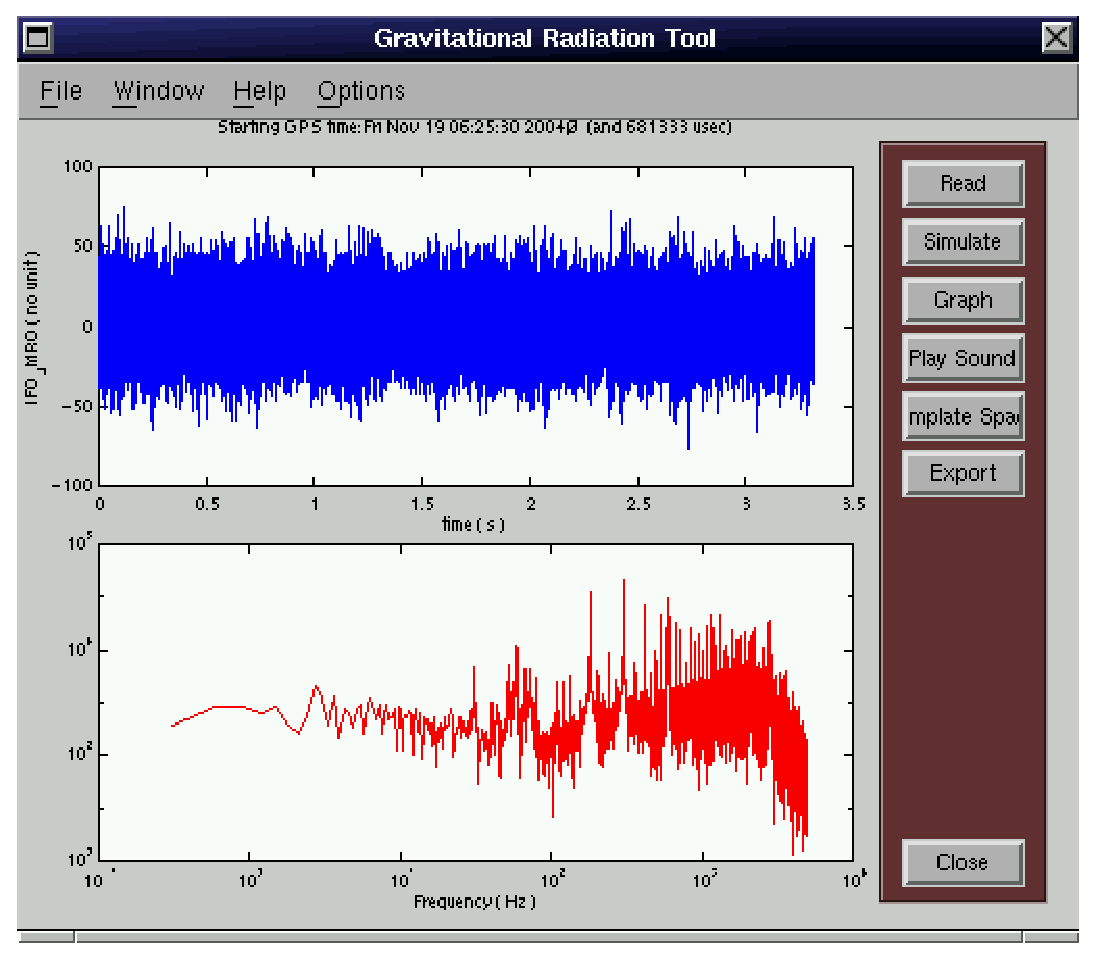
\epsfig{file=Figures/fig_tfspace.eps,width=6in}
\caption{ \label{f:tfspace}
Viewing data in the time and frequency domain}
\end{center}
\end{figure}
%%%%%%%%%%%%%%%%%%%%%%%%%%%%%%%%%%%%%%%%%%%%%%%%%%%%%%%%%%%%%%%%%%%%%%%%%%%%%%%%
The data plotted will only appear if you press \texttt{Graph} and then
enter a time-span for which you want to look at data. The \texttt{Play Sound} button
will playback the data from your speakers. The \texttt{Export} button
allows you to export time domain data to a \texttt{*.au} sound file or
the Matlab workspace. If you export the data to the workspace it will be
preserved there even if you close \texttt{GRtool}. Then you can do with
it what you like as it will behave as any other normal Matlab variable.

Pressing \texttt{Template Space} will change your view from time/frequency
space to template space. Your window will change to look like figure
\ref{f:tmplt_startup}.

%%%%%%%%%%%%%%%%%%%%%%%%%%%%%%%%%%%%%%%%%%%%%%%%%%%%%%%%%%%%%%%%%%%%%%%%%%%%%%
%tmplt_startup.gif 
\begin{figure}[h]
\index{colorpage}
\begin{center}
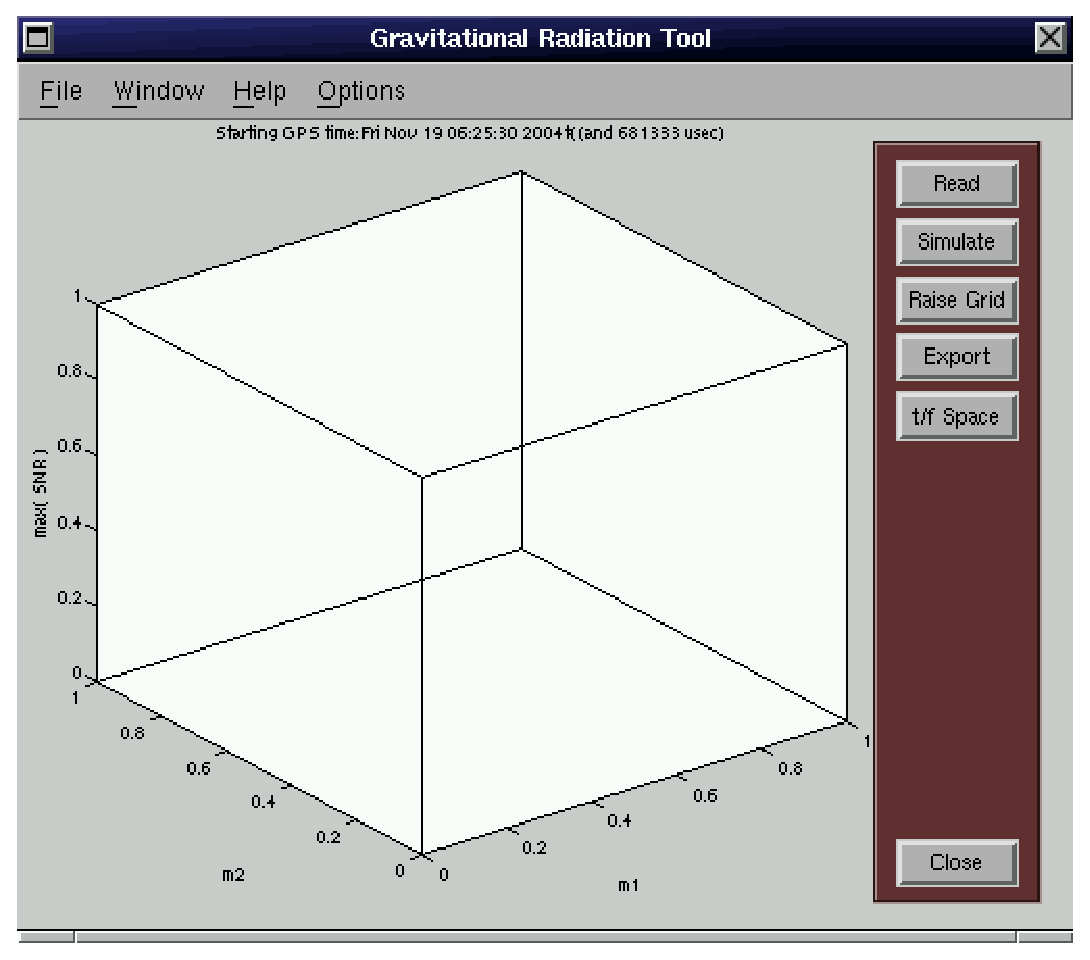
\epsfig{file=Figures/fig_tmplt_startup.eps,width=6in}
\caption{ \label{f:tmplt_startup}
The initial template space window}
\end{center}
\end{figure}
%%%%%%%%%%%%%%%%%%%%%%%%%%%%%%%%%%%%%%%%%%%%%%%%%%%%%%%%%%%%%%%%%%%%%%%%%%%%%%%%

From template space you can observe the effect of the data set on a grid of
matched filters. You can always go back to see the data in time/frequency
space by pressing \texttt{t/f Space}. Similarly from time/frequency space, you
can always go to template space by pressing \texttt{Template Space}.

When you enter template space you will also see the template space control
panel shown in figure \ref{f:tmplt_control}.
%%%%%%%%%%%%%%%%%%%%%%%%%%%%%%%%%%%%%%%%%%%%%%%%%%%%%%%%%%%%%%%%%%%%%%%%%%%
%tmplt_control.gif
\begin{figure}[h]
\index{colorpage}
\begin{center}
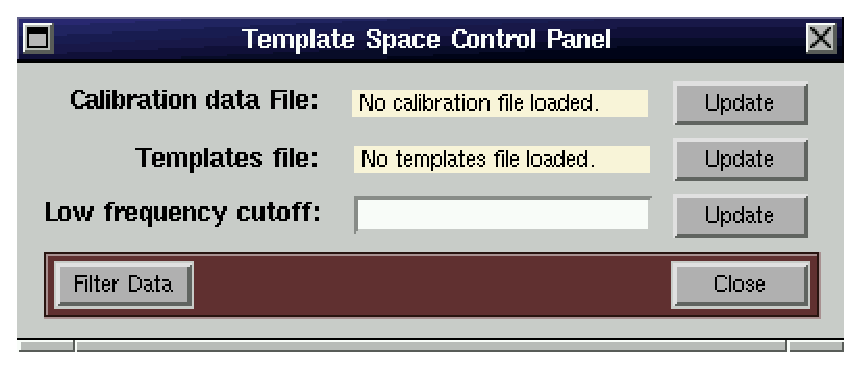
\epsfig{file=Figures/fig_tmplt_control.eps,width=5in}
\caption{ \label{f:tmplt_control}
The template space control panel}
\end{center}
\end{figure}
%%%%%%%%%%%%%%%%%%%%%%%%%%%%%%%%%%%%%%%%%%%%%%%%%%%%%%%%%%%%%%%%%%%%%%%%%%%%

With this window you control the files and parameters used for any filtering
you do. You can always change a parameter or file by pressing it's
corresponding \texttt{Update} button. The calibration file must be a text file
with one column of numbers which are the swept sine calibration information
contained in the \texttt{fri} array returned by the function
\texttt{fget\_ch} or it's Matlab counterpart \texttt{mxFget\_ch}. You can
generate the calibration files using the \texttt{getfri} function as described
in section \ref{sss:getfri}. The templates file must be a two column text file.
The two columns are the $\left(  m_{1},m_{2}\right)  $ pairs that you wish to
include in your grid of filters. There is a very detailed discussion of what
$\left(  m_{1},m_{2}\right)  $ pairs to use in section \ref{s:binary-search}.
There is a sample templates file in 
\texttt{\$GRASP/src/examples/examples\_binary-search/templates.ascii} where
\texttt{\$GRASP} is your GRASP root directory. The \texttt{Low frequency
cutoff} is the lowest frequency at which the detector you are interested in
can operate. This value must be entered in Hz.

After you have specified the necessary files and low frequency cutoff you can
filter your data by pressing \texttt{Filter Data}. As the filters are being
generated and compared against the data you will see lots of text streaming by
in the workspace. This text will say something similar to the following:
\begin{verbatim}
GRASP (page-173.caltech.edu): Message from function phase_frequency() 
at line number 536 of file ''pN_chirp.c''.
Frequency evolution no longer monotonic.
Phase evolution terminated at frequency and step: 466.659027 4347
Terminating chirp. Termination code set to: 1201
Returning to calling routine.
$Id: man_GRtoolbox.tex,v 1.3 1999/09/06 17:37:17 ballen Exp $
$Name: RELEASE_1_9_8 $
max snr: 2.56 offset: 24659 variance: 0.95574
max snr: 2.56 offset: 2376 variance: 0.96000
max snr: 2.70 offset: 10504 variance: 0.95999
Done filtering 32768 data points through 20 filters
\end{verbatim}
The final line will always tell you how many data points and how many filters
were used.

After you filter the data you can visualize the response of the filters by
pressing \texttt{Raise Grid} in the main window. A typical response is shown
in figure \ref{f:filter_response}. The color of the plotted points is based on
the time at which that specific filter had the greatest SNR. The colors range
from pure blue to pure black. The darker the color the earlier the time.

%%%%%%%%%%%%%%%%%%%%%%%%%%%%%%%%%%%%%%%%%%%%%%%%%%%%%%%%%%%%%%%%%%%%%%%%%%%%%%
%filter_response.gif 
\begin{figure}[h]
\index{colorpage}
\begin{center}
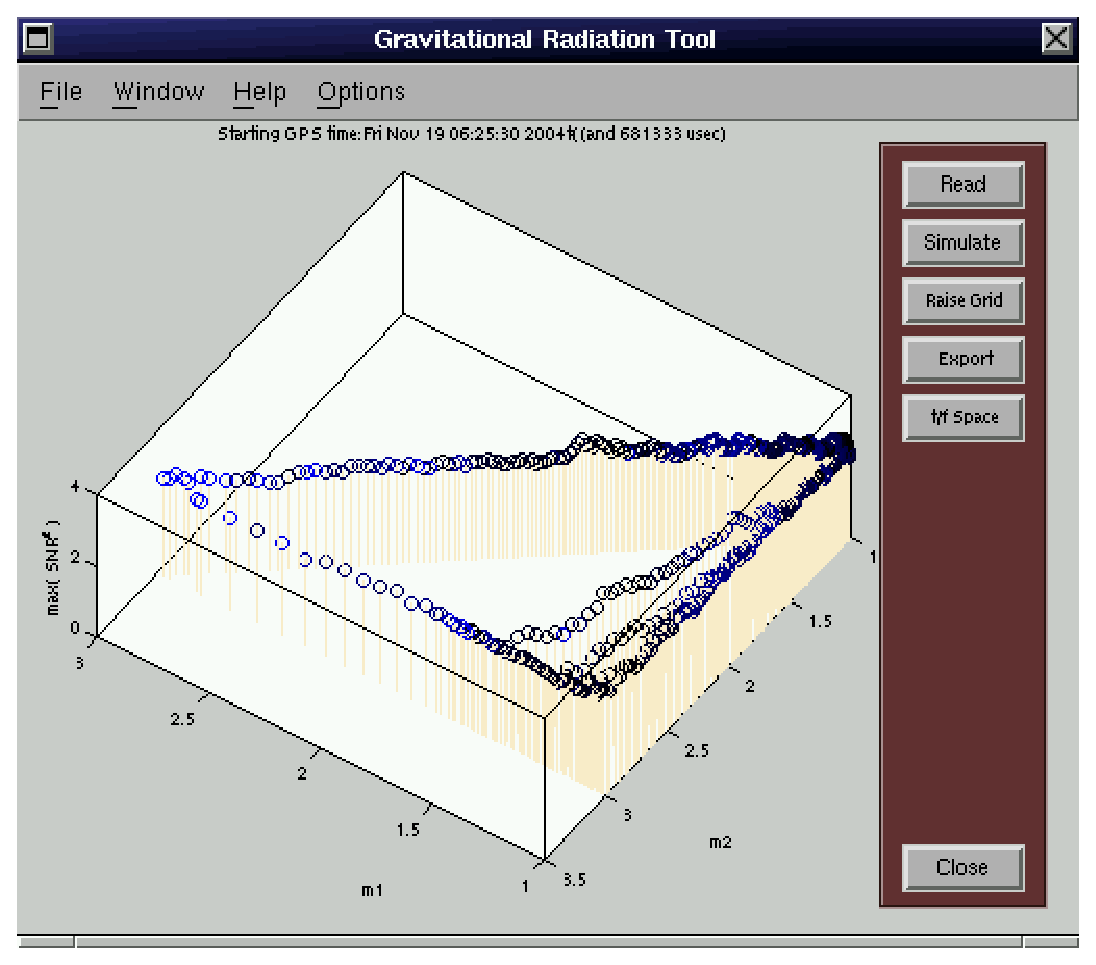
\epsfig{file=Figures/fig_filter_response.eps,width=6in}
\caption{ \label{f:filter_response}
Viewing the data in template space}
\end{center}
\end{figure}
%%%%%%%%%%%%%%%%%%%%%%%%%%%%%%%%%%%%%%%%%%%%%%%%%%%%%%%%%%%%%%%%%%%%%%%%%%%%%%

Figure \ref{f:filter_response_inject} shows the response of the filters when a
simulated inspiral of $m_{1}=m_{2}=1.4M_{\odot}$ has been injected into the
data stream.
%%%%%%%%%%%%%%%%%%%%%%%%%%%%%%%%%%%%%%%%%%%%%%%%%%%%%%%%%%%%%%%%%%%%%%%%%%%%%%%
%filter_response_inject.gif 
\begin{figure}[h]
\index{colorpage}
\begin{center}
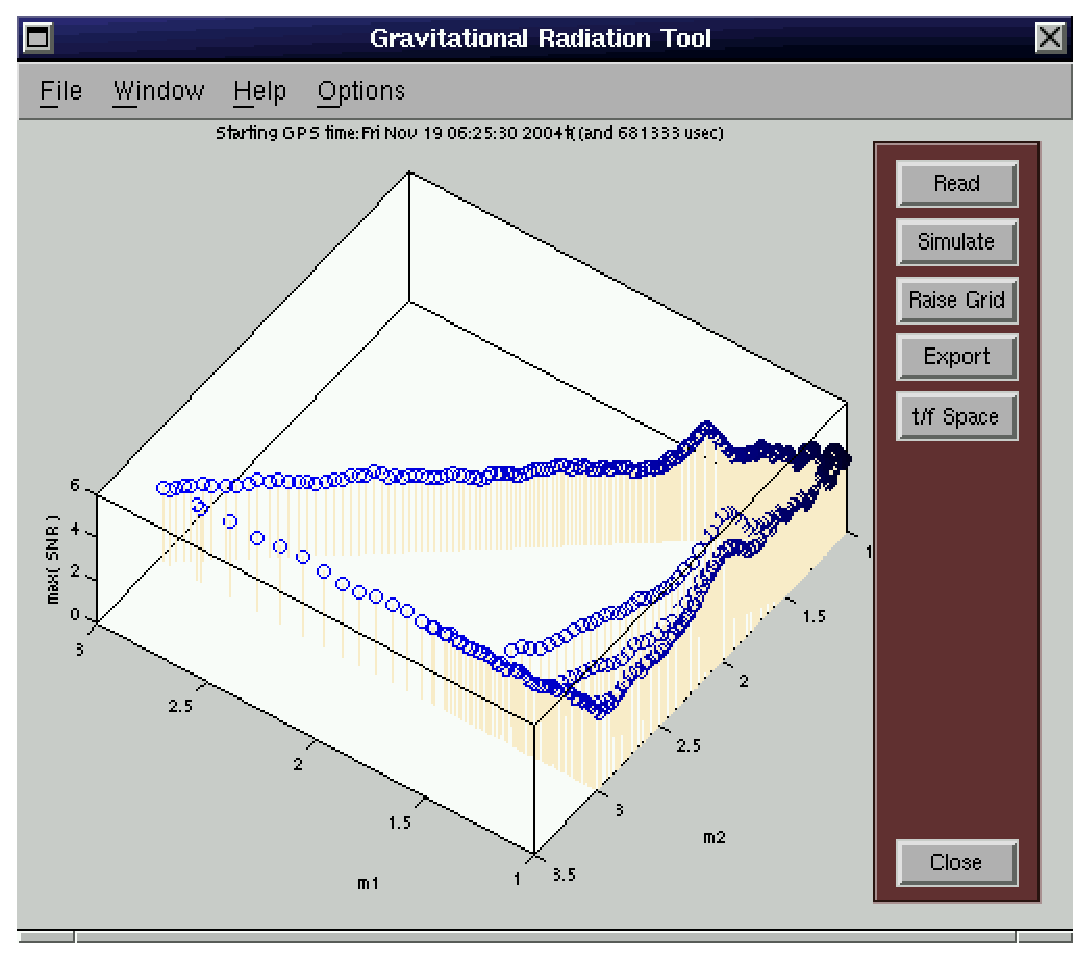
\epsfig{file=Figures/fig_filter_response_inject.eps,width=6in}
\caption{ \label{f:filter_response_inject}
An artificial inspiral detection of $m_{1}=m_{2}=1.4M_{\odot}$}
\end{center}
\end{figure}
%%%%%%%%%%%%%%%%%%%%%%%%%%%%%%%%%%%%%%%%%%%%%%%%%%%%%%%%%%%%%%%%%%%%%%%%%%%%%%%%%

You can clearly see the filters responding. Notice also that the colors have a
well defined pattern in this image. If you press \texttt{Export} in this
window you will be able to export the arrays $m_{1},m_{2},$ \texttt{max(SNR)}
and \texttt{timestart} to the workspace. The \texttt{timestart} array contains
the time in seconds (relative to the first time stamp) at which the
corresponding filter had a maximum. A more detailed description of the array
\texttt{timestart} can be found in the description of the function
\texttt{find\_chirp} in section \ref{ss:find_chirp}.

\subsection{Functions}
\label{ss:GRtoolboxFunctions}

Bellow is a list of the functions available to you for use within Matlab. The
majority of the functions are ports of other GRASP functions. These have names that
are identical to their GRASP versions except their first letter is capitalized
and they are prefixed by \texttt{mx}. For example the Matlab version of the
GRASP function \texttt{make\_filters} is called \texttt{mxMake\_filters}.
These functions differ from their GRASP counterparts only
in their calling methods. \textbf{Warning}: you must be careful that you have
set any environment variables required by the GRASP functions \emph{before}
starting Matlab. If you have not, calling functions that require these
variables will abort Matlab and you will lose any data you had stored in the
workspace! Use these functions cautiously!

\subsubsection{Function: {\tt frextract}}
\label{sss:frextract}

\texttt{[a,t,f,t0,t0s,c,u,more]=frextract(file,channel,firstframe,nframes)}

This function is part of the standard frame library distribution.
Extracts data from a frame file. See Section 6 of \cite{frame}
for further documentation.

\subsubsection{Function: {\tt getfri}}
\label{sss:getfri}

\texttt{getfri('fri.ascii'}) Generates calibration files for use with
\texttt{GRtool}. \texttt{W}ill create a file called \texttt{fri.ascii}. This
function requires that you have set the environment variable
\texttt{GRASP\_FRAMEPATH} to point to the data file from which you want
calibration data. This function calls the \texttt{mxFget\_ch} function once.
See the warning about its use in section \ref{sss:mxFget_ch}.

\begin{description}
\item{Author:} Steve Drasco, steve.drasco@cornell.edu
\item{Comments:} None.
\end{description}


\subsubsection{Function: {\tt inspfilt}}
\label{sss:inspfilt}

\texttt{[snr\_max,timestart]=inspfilt(m1,m2,data,srate,flo,fri)}

Filters data through a grid of matched filters.

\begin{description}
\item{\tt m1 and m2:} equal length vectors specifying the
filters to use.

\item{\tt data:} vector containing the data to be filtered.

\item{\tt srate:} sampling frequency of the data in Hz.

\item{\tt flo:} low frequency cutoff for the detector in Hz.

\item{\tt fri:} vector containing the calibration data from the instrument.

\item{\tt snr\_max:} vector with the same length as \texttt{m1} and
\texttt{m2}. It contains the maximum value of the SNR for each filter.

\item{\tt timestart:} vector with the same length as \texttt{snr\_max}
which specifies the time in seconds (relative to the first time stamp) at
which the corresponding filter reached the value contained in \texttt{snr\_max}
\end{description}

\begin{description}
\item{Author:} Steve Drasco, steve.drasco@cornell.edu
\item{Comments:} None.
\end{description}

\subsubsection{Function: {\tt mxAvg\_inv\_spec}}
\label{sss:max_avg_inv_spec}

\texttt{[mean\_pow\_spec,twice\_inv\_noise,norm]}=\texttt{mxAvg\_inv\_spec(flo,srate,n,}
\texttt{decay,norm,htilde)}

All variables are identical to their description in section \ref{ss:avg_inv_spec}.

\begin{description}
\item{Author:} Steve Drasco, steve.drasco@cornell.edu
\item{Comments:} None.
\end{description}

\subsubsection{Function: {\tt mxChirp\_filters}}
\label{sss:mxChirp_filters}

\texttt{[Max\_Freq\_Actual,h\_c,h\_s,steps\_filld,clscnc\_time]=mxChirp\_filters} \\
\texttt{(m1,m2,spin1,spin2,n\_phaseterms,phaseterms,Initial\_Freq,} \\
\texttt{Max\_Freq\_Rqst,Sample\_Time,steps\_alloc,err\_cd\_sprs)}

All variables are identical to their description in section \ref{ss:chirp_filters}.

\begin{description}
\item{Author:} Steve Drasco, steve.drasco@cornell.edu
\item{Comments:} None.
\end{description}

\subsubsection{Function: {\tt mxCompute\_match}}
\label{sss:mxCompute_match}

\texttt{[outvalue]=mxCompute\_match(m1,m2,ch0tilde,ch90tilde,} \\
\texttt{inverse\_discance\_scale,twice\_inv\_noise,flo,s\_n0,s\_n90,npoint,} \\
\texttt{srate,err\_cd\_sprs,order)}

All variables are identical to their description in section \ref{ss:compute_match}.

\begin{description}
\item{Author:} Steve Drasco, steve.drasco@cornell.edu
\item{Comments:} None.
\end{description}

\subsubsection{Function: {\tt mxCorrelate}}
\label{sss:mxCorrelate}

\texttt{[s]=mxCorrelate(h,c,r,n)}

All variables are identical to their description in section \ref{ss:correlate}.

\subsubsection{Function: {\tt mxDetector\_site}}
\label{sss:mxDetector_site}

\texttt{[site\_parameters,site\_name,noise\_file,whiten\_file]=mxDetector\_site} \\
\texttt{(detectors\_file,site\_choice)}

All variables are identical to their description in section \ref{subsec:detector_site}.

\begin{description}
\item{Author:} Steve Drasco, steve.drasco@cornell.edu
\item{Comments:} None.
\end{description}

\subsubsection{Function: {\tt mxFget\_ch}}
\label{sss:mxFget_ch}

\texttt{[fgetoutput]=mxFget\_ch(fgetinput)}

This function does not behave properly. GRASP treats Matlab as the calling
function so it has no way of knowing when you want to reset your search. Be
\emph{especially} cautious if you use this function. Most of the input and
output structures are the same---however since there are slight difference the
full descriptions are given below.

\begin{description}
\item{\tt fgetinput.npoint:} the number of data points you want to get

\item{\tt fgetinput.inlock:} 1 means get only locked data 0 means get
both locked and unlocked data

\item{\tt fgetinput.seek:} 1 means operate in seek mode (do not return
data) 0 means return data

\item{\tt fgetinput.calibrate:} 1 means return calibration data 0 means
do not return calibration data

\item{\tt fgetinput.nchan:} number of channels to read from

\item{\tt fgetinput.chnames:} cell array whose elements are strings
containing the channel names

\item{\tt fgetoutput.tstart:} time stamp of the first point output in
channel \texttt{chnames\{1\}}

\item{\tt fgetoutput.srate}] sample rate at which data was recorded

\item{\tt fgetoutput.npoint:} \texttt{npoint(i)}is the number of points
returned for channel \texttt{chnames\{i\}}

\item{\tt fgetoutput.ratios:} \texttt{ratios(i)} is the sample rate of
channel \texttt{chnames\{1\}} divided by the sample rate of channel \texttt{chnames\{i\}}

\item{\tt fgetoutput.discarded:} number of points discarded from channel \texttt{chnames\{1\}}

\item{\tt fgetoutput.tfirst:} the time stamp of the first point returned
in the first call to \texttt{mxFget\_ch}

\item{\tt fgetoutput.dt:} \texttt{tstart-tfirst}

\item{\tt fgetoutput.lostlock:} time at which we lost lock (if searching
for locked segments only)

\item{\tt fgetoutput.lastlock:} time at which we last regained lock (if
searching for locked segments only)

\item{\tt fgetoutput.returnval:} 0 if unable to satisfy the request, 1 if
request is satisfied by beginning new locked or continuous-in-time section, 2
if the data returned is part of an ongoing locked or continuous-in-time sequence

\item{\tt fgetoutput.frinum:} three times the number of frequency values
for which re are returning static calibration information.

\item{\tt fgetoutput.fri:} calibration data \texttt{fri(1)}$=f_{0},$
\texttt{fri(2)}$=r_{0},$ \texttt{fri(3)}$=i_{0},$ \texttt{fri(4)}$=f_{1},$
\texttt{fri(5)}$=r_{1},$ \texttt{fri(6)}$=i_{1}$ $\cdots$ (see section 4.7)

\item{\tt fgetoutput.tcalibrate:} time at which current calibration data
became valid

\item{\tt fgetoutput.locklow:} minimum value (inclusive) for ``in-lock''
in the lock channel, \\
set only if \texttt{fgetinput.inlock} is nonzero

\item{\tt fgetoutput.lockhi:} maximum value (inclusive) for ``in-lock''
in the lock channel, \\
set only if \texttt{fgetinput.inlock} is nonzero

\item{\tt fgetoutput.data:} a cell array. \texttt{fgetoutput.data\{i\}}
is a vector containing the returned data for channel \texttt{chnames\{i\}}
\end{description}

\begin{description}
\item{Author:} Steve Drasco, steve.drasco@cornell.edu
\item{Comments:}
A possible fix to this function would be to write a reset function for \texttt{fget\_ch}.
The reset function would tell \texttt{fget\_ch} that we are going to start a new data 
input run. Another possible fix would be to add a field \texttt{fgetinput.reset} which 
could reset the function.
\end{description}

\subsubsection{Function: {\tt mxFind\_chirp}}
\label{sss:mxFind_chirp}

\texttt{[output0,output90,offset,snr\_max,c0,c90,var]=mxFind\_chirp(htilde,} \\
\texttt{ch0tilde,ch90tilde,twice\_inv\_noise,n0,n90,n,chirplen)}

All variables are identical to their description in section \ref{ss:find_chirp}.

\begin{description}
\item{Author:} Steve Drasco, steve.drasco@cornell.edu
\item{Comments:} None.
\end{description}

\subsubsection{Function: {\tt mxFreq\_inject\_chirp}}
\label{sss:mxFreq_inject_chirp}

\texttt{[htilde]=mxFreq\_inject\_chirp(c0,c90,offset,invMpc,ch0tilde,}
\texttt{ch90tilde,n)}

All variables are identical to their description in section \ref{ss:freq_inject_chirp}.

\begin{description}
\item{Author:} Steve Drasco, steve.drasco@cornell.edu
\item{Comments:} None.
\end{description}

\subsubsection{Function: {\tt mxGRcalibrate}}
\label{sss:mxGRcalibrate}

\texttt{[complex]=mxGRcalibrate(fri,frinum,num,srate,method,order)}

All variables are identical to their description in section \ref{ss:GRcalibrate}.

\begin{description}
\item{Author:} Steve Drasco, steve.drasco@cornell.edu
\item{Comments:} None.
\end{description}

\subsubsection{Function: {\tt mxGRnormalize}}
\label{sss:mxGRnormalize}

\texttt{[response]=mxGRnormalize(fri,frinum,npoint,srate)}

All variables are identical to their description in section \ref{s:normalizeF}.

\begin{description}
\item{Author:} Steve Drasco, steve.drasco@cornell.edu
\item{Comments:} None.
\end{description}

\subsubsection{Function: {\tt mxM\_and\_eta}}
\label{sss:mxM_and_eta}

\texttt{[m,eta]=mxM\_and\_eta(tau0,tau1,Mmin,Mmax,pf)}

All variables are identical to their description in section \ref{ss:m_and_eta}.

\begin{description}
\item{Author:} Steve Drasco, steve.drasco@cornell.edu
\item{Comments:} None.
\end{description}

\subsubsection{Function: {\tt mxMake\_filters}}
\label{sss:mxMake_filters}

\texttt{[ch1,ch2,filled,t\_coal]=mxMake\_filters(m1,m2,fstart,length,srate,} \\
\texttt{err\_cd\_sprs,order)}

All variables are identical to their description in section \ref{ss:make_filters}.

\begin{description}
\item{Author:} Steve Drasco, steve.drasco@cornell.edu
\item{Comments:} None.
\end{description}

\subsubsection{Function: {\tt mxMatch\_cubic}}
\label{sss:mxMatch_cubic}

\texttt{[semimajor,semiminor,theta,mcoef,outval]=mxMatch\_cubic(m1ref,m2ref,} \\
\texttt{mathcont,order,srate,flo,ftau,noisefile)}

All variables are identical to their description in section \ref{ss:match_cubic}.

\begin{description}
\item{Author:} Steve Drasco, steve.drasco@cornell.edu
\item{Comments:} None.
\end{description}

\subsubsection{Function: {\tt mxOrthonormalize}}
\label{sss:mxOrthonormalize}

\texttt{[n0,n90,ch90tilde]=mxOrthonormalize(ch0tilde,ch90tilde,} \\
\texttt{twice\_inv\_noise,n)}

All variables are identical to their description in section \ref{ss:orthonormalize}.

\begin{description}
\item{Author:} Steve Drasco, steve.drasco@cornell.edu
\item{Comments:} None.
\end{description}

\subsubsection{Function: {\tt mxPhase\_frequency}}
\label{sss:mxPhase_frequency}

\texttt{[Max\_Freq\_Actual,phase,frequency,steps\_filld,clscnc\_time]=mxPhase\_frequency} \\
\texttt{(m1,m2,spin1,spin2,n\_phaseterms,phaseterms,} \\
\texttt{Initial\_Freq,Max\_Freq\_Rqst,Sample\_Time,steps\_alloc,err\_cd\_sprs)}

All variables are identical to their description in section \ref{ss:phase_frequency}.

\begin{description}
\item{Author:} Steve Drasco, steve.drasco@cornell.edu
\item{Comments:} None.
\end{description}

\subsubsection{Function: {\tt mxSp\_filters}}
\label{sss:mxSp_filters}

\texttt{[ch1,ch2,f\_c]=mxSp\_filters(m1,m2,fstart,n,srate,t\_c,order)}

All variables are identical to their description in section \ref{ss:sp_filters}.

\begin{description}
\item{Author:} Steve Drasco, steve.drasco@cornell.edu
\item{Comments:} None.
\end{description}

\subsubsection{Function: {\tt mxSplitup}}
\label{sss:mxSplitup}

\texttt{[indices]=mxSplitup(working,template,r,n,total,p)}

All variables are identical to their description in section \ref{ss:splitup}.

\begin{description}
\item{Author:} Steve Drasco, steve.drasco@cornell.edu
\item{Comments:} None.
\end{description}

\subsubsection{Function: {\tt mxSplitup\_freq}}
\label{sss:mxSplitup_freq}

\texttt{[indices,stats,working,htilde]=mxSplitup\_freq(c0,c90,chirp0,chirp90,} \\
\texttt{norm,twice\_inv\_noise,n,offset,p)}

All variables are identical to their description in section \ref{ss:splitup_freq}.

\begin{description}
\item{Author:} Steve Drasco, steve.drasco@cornell.edu
\item{Comments:} None.
\end{description}

\subsubsection{Function: {\tt mxSplitup\_freq2}}
\label{sss:mxSplitup_freq2}

\texttt{[indices,stats,working,htilde]=mxSplitup\_freq2(c0,c90,chirp0,chirp90,} \\
\texttt{norm,twice\_inv\_noise,n,offset,p)}

All variables are identical to their description in section \ref{ss:splitup_freq2}.

\begin{description}
\item{Author:} Steve Drasco, steve.drasco@cornell.edu
\item{Comments:} None.
\end{description}

\subsubsection{Function: {\tt mxTau\_of\_mass}}
\label{sss:mxTau_of_mass}

\texttt{[tau0,tau1]=mxTau\_of\_mass(m1,m2,pf)}

All variables are identical to their description in section \ref{ss:tau_of_mass}.

\begin{description}
\item{Author:} Steve Drasco, steve.drasco@cornell.edu
\item{Comments:} None.
\end{description}

\subsubsection{Function: {\tt mxTemplate\_area}}
\label{sss:mxTemplate_area}

\texttt{[Grid,area]=mxTemplate\_area(Grid)}

An empty scope structure can be made with the command
\texttt{Grid=scope\_structure}. All fields are identical to their
description in section \ref{ss:area}.

\subsubsection{Function: {\tt mxTime\_inject\_chirp}}
\label{sss:mxTime_inject_chirp}

\texttt{[data,work]=mxTime\_inject\_chirp(c0,c90,offset,invMpc,chirp0,chirp90,} \\
\texttt{response,data,n)}

All variables are identical to their description in section \ref{ss:time_inject_chirp}.

\begin{description}
\item{Author:} Steve Drasco, steve.drasco@cornell.edu
\item{Comments:} None.
\end{description}

\subsubsection{Function: {\tt mxUrlopen}}
\label{sss:mxUrlopen}

\texttt{mxUrlopen('URL','filename')}

This function gets the file found at \texttt{URL} and writes it to a local
file \texttt{filename}.

\begin{description}
\item{Authors:} Steve Drasco, steve.drasco@cornell.edu
\item{Comments:}
This program is an adaptation of the program \texttt{urlopen.c} by 
Mark Niedengard, Roy Williams, and George Kremenek.
\end{description}

\subsection{Examples}
\label{ss:GRtoolboxExamples}

The code for the following examples can be found in the directory \\
\texttt{\$GRASP/src/examples/examples\_GRtoolbox}.

\subsubsection{Example: {\tt print\_ssF}}
\label{sss:print_ssF}

A Matlab version of the \texttt{print\_ssF} example found in section \ref{ss:print_ssF}.

\begin{verbatim}
function print_ssF();
% PRINT_SSF
%	A Matlab version of the GRASP example: print_ssF.
%	Example run: print_ssF
%
% Steve Drasco
% Summer 1998

% get some data
fgetinput.npoint = 256;
fgetinput.nchan = 1;
fgetinput.chnames = {'IFO_DMRO'};
fgetinput.inlock = 0;
fgetinput.seek = 1;
fgetinput.calibrate = 1;
fgetoutput = mxFget_ch(fgetinput);

% call mxGRcalibrate
srate = fgetoutput.srate;
npoint = 4096;
cplx=mxGRcalibrate(fgetoutput.fri,fgetoutput.frinum,npoint,srate,2,0);

% plot output
freq=1:npoint/2;
freq = freq*srate/npoint;
imaginary = cplx(2*(1:npoint/2));
real = cplx(2*(1:npoint/2)+1);
plot(freq, real, 'b', freq, imaginary, 'r');
\end{verbatim}

\subsubsection{Example: {\tt power\_spectrumF}}
\label{sss:power_spectrumF}

A Matlab version of the \texttt{power\_spectrumF} example in section \ref{ss:power_spectrumF}.

\begin{verbatim}
function [fgetoutput, response]=power_spectrumF()
% POWER_SPECTRUMF
%	A Matlab version of the GRASP example: power_spectrumF.
%	Example run: [fgetoutput, response]=power_spectrumF;
%
% Steve Drasco
% Summer 1998

npoint = 65536;
fgetinput.nchan = 1;
fgetinput.chnames = {'IFO_DMRO'};
fgetinput.inlock = 1;
fgetinput.npoint = npoint;
fgetinput.calibrate = 1;

% I won't skip any data
fgetinput.seek = 0;
fgetoutput = mxFget_ch(fgetinput);
srate = fgetoutput.srate;
data = fft(fgetoutput.data{1});
response=mxGRnormalize(fgetoutput.fri,fgetoutput.frinum,npoint,srate);

% one-sided power-spectrum normalization, to get meters/rHz
factor = sqrt(2/(srate*npoint));

% frequency
freq = (1:(npoint/2)-1)*srate/npoint;

% real and imaginary parts of tilde c0
c0_real = real( data( 2:npoint/2 ) );
c0_imag = imag( data( 2:npoint/2 ) );

% real and imaginary parts of R
res_real = response(   1 + 2*( 2:npoint/2  )   );
res_imag = response(   2 + 2*( 2:npoint/2  )   );

% real and imaginary parts of tilde dl
dl_real = c0_real.*res_real - c0_imag.*res_imag;
dl_imag = c0_real.*res_imag + c0_imag.*res_real;
spectrum = factor * sqrt(dl_real.^2 + dl_imag.^2);

% plot the results
loglog(freq, spectrum);
xlabel('frequency (Hz)');
ylabel('noise m/(Hz^1/2)'); 
\end{verbatim}

\subsubsection{Example: {\tt phase\_evoltn}}
\label{sss:phase_evoltn}

A Matlab version of the \texttt{phase\_evoltn} example found in section \ref{ss:phase_evoltn}.

\begin{verbatim}
function phase_evoltn()
% PHASE_EVOLUTION
%	A Matlab version of the GRASP example: phase_evolution.
%	Example run: phase_evolution
%
% Steve Drasco
% Summer 1998

m1 = 1.4;
m2 = 1.4;
spin1 = 0;
spin2 = 0;
n_phaseterms = 5;
Initial_Freq = 60;
Max_Freq_Rqst = 2000;
Sample_Time = 1/9868.4208984375;
err_cd_sprs = 0;
phaseterms = [1 0 1 1 1];

[Max_Freq_Actual,phase,frequency,steps_filld,...
clscnc_time]=mxPhase_frequency(m1,m2,spin1,spin2,n_phaseterms,phaseterms,...
Initial_Freq,Max_Freq_Rqst,Sample_Time,[],err_cd_sprs);

time = (1:steps_filld) * Sample_Time;

subplot(2,1,1)
	plot(time, phase,'b');
	xlabel('time (s)');
	ylabel('phase');
subplot(2,1,2)
	plot(time, frequency,'r');
        xlabel('time (s)');
        ylabel('frequency (Hz)');
\end{verbatim}

\subsubsection{Example: {\tt filters}}
\label{sss:filters}

A Matlab version of the \texttt{filters} example found in section \ref{ss:filters}.

\begin{verbatim}
function filters()
% FILTERS
%	A Matlab version of the GRASP example: filters.
%	Example run: filters
%
% Steve Drasco
% Summer 1998

m1 = 1.4;
m2 = 1.4;
spin1 = 0;
spin2 = 0;
n_phaseterms = 5;
Initial_Freq = 60;
Max_Freq_Rqst = 2000;
Sample_Time = 1/9868.4208984375;
err_cd_sprs = 0;
phaseterms = [1 0 1 1 1];

[Max_Freq_Actual,h_c,h_s,steps_filld,clscnc_time]=mxChirp_filters(m1,m2,...
spin1,spin2,n_phaseterms,phaseterms,Initial_Freq,Max_Freq_Rqst,Sample_Time,...
[],err_cd_sprs);

time = (1:steps_filld) * Sample_Time;

plot(time, h_c,'b', time, h_s,'r');
xlabel('time (s)');
ylabel('h_c and h_s');
\end{verbatim}

\subsubsection{Example: {\tt area}}
\label{sss:area}

A Matlab version of the \texttt{area} example found in section \ref{ss:area}.

\begin{verbatim}
function [Gridout, out] = area()
% AREA
%	A Matlab version of the example: area in GRASP.
%	Example run: [Gridout, out] = area;
%
% Steve Drasco
% Summer 1998

Grid = scope_structure;

Grid.m_mn = 0.8;
Grid.m_mx = 50.0;
Grid.f_start = 140.0;

[Gridout, out] = mxTemplate_area(Grid);
\end{verbatim}

\subsubsection{Example: {\tt match\_fit}}
\label{sss:match_fit}

A Matlab version of the \texttt{match\_fit} example found in section \ref{ss:match_fit}.

\begin{verbatim}
function [semimajor,semiminor,theta,mcoef,tstp]=match_fit(m1,m2,matchcont,...
order)
% MATCH_FIT
%	A Matlab version of the GRASP example: match_fit.
%	Example run: [semimajor,semiminor,theta,mcoef,tstp]=match_fit(m1,m2,...
%		     matchcont,order)
%
% Steve Drasco
% Summer 1998

srate = 50000;
detector_num = 15;
flo = 120;
ftau = 140;

[site_parameters,site_name,noise_file,...
whiten_file]=mxDetector_site('detectors.dat',detector_num);

[semimajor,semiminor,theta,mcoef,tstp]=mxMatch_parab(m1,m2,matchcont,...
order,srate,flo,ftau,noise_file);
if tstp
	semimajor
	semiminor
	theta
	mcoef
elseif ~tstp
	[semimajor,semiminor,theta,mcoef,tstp]=mxMatch_parab(m1,m2,matchcont,order,...
	srate,flo,ftau,noise_file);
	semimajor
        semiminor
        theta
        mcoef
end
\end{verbatim}

\subsubsection{Example: {\tt readfri}}
\label{sss:readfri}

Reads the swept sine calibration information from a frame and returns it in an
\texttt{fgetoutput} structure.

\begin{verbatim}
function fgetoutput=readfri()
% READFRI
%	This program reads the calibaration data from a frame file.
%	Example run: fgetoutput=readfri
%
% Steve Drasco
% Summer 1998

fgetinput.npoint=65536;
fgetinput.inlock=1;
fgetinput.seek=0;
fgetinput.calibrate=1;

fgetinput.nchan=1;
fgetinput.chnames={'IFO_DMRO'};

%fgetinput.chnames={'IFO_DMRO','IFO_DCDM'};
%fgetinput.nchan=2;

fgetoutput=mxFget_ch(fgetinput);
\end{verbatim}


\subsubsection{Example: {\tt oneFget}}
\label{sss:oneFget}

Calls the GRASP function \texttt{fget\_ch} once to read data from a file. You
can edit the comments to retrieve data from one or two channels.

\begin{verbatim}
function fgetoutput=oneFget()
% ONEFGET
%	This Program uses the GRASP function fget_ch() once and returns the output
%
% Steve Drasco
% Summer 1998

fgetinput.npoint=296000;
fgetinput.inlock=1;
fgetinput.seek=0;
fgetinput.calibrate=1;

%fgetinput.nchan=1;
%fgetinput.chnames={'IFO_DMRO'}

fgetinput.chnames={'IFO_DMRO','IFO_DCDM'};
fgetinput.nchan=2;

fgetoutput=mxFget_ch(fgetinput);
\end{verbatim}

\subsubsection{Example: {\tt twoFget}}
\label{sss:twoFget}

This example works just like \texttt{oneFget} except that it uses the GRASP
function \texttt{fget\_ch} twice.

\begin{verbatim}
function fgetoutput=twoFget()
% TWOFGET
%	This program uses the GRASP function fget_ch() twice and returns the output.
%
% Steve Drasco
% Summer 1998

fgetinput.npoint = 296000;
fgetinput.inlock = 1;
fgetinput.seek = 0;
fgetinput.calibrate = 1;

% uncomment these to get one channel
fgetinput.nchan=1;
fgetinput.chnames={'IFO_DMRO'}

% uncomment these to get two channels
%fgetinput.chnames={'IFO_DMRO','IFO_DCDM'};
%fgetinput.nchan=2;

for i = 1:2
	fgetoutput = mxFget_ch(fgetinput);
end
\end{verbatim}
